%=============================================================================
%=============================================================================

\chapter{Structured-Grid System Interface (Struct)}
\label{ch-Struct}

In order to get access to the most efficient and scalable solvers for
scalar structured-grid applications, users should use the
\code{Struct} interface described in this chapter.  This interface
will also provide access (this is not yet supported) to solvers in
\hypre{} that were designed for unstructured-grid applications and
sparse linear systems in general.  These additional solvers are
usually provided via the unstructured-grid interface (\code{FEI}) or
the linear-algebraic interface (\code{IJ}) described in Chapters
\ref{ch-FEI} and \ref{ch-IJ}.

Figure~\ref{fig-struct-example} gives an example of the type of grid
currently supported by the \code{Struct} interface.  The interface
uses a finite-difference or finite-volume style, and currently
supports only scalar PDEs (i.e., one unknown per gridpoint).
\begin{figure}
\centering
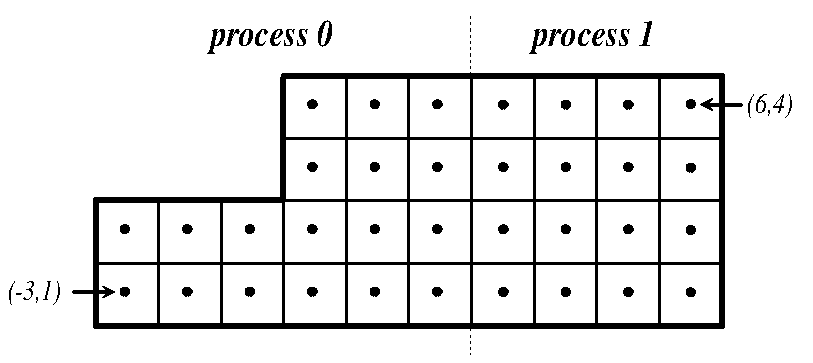
\includegraphics[width=.5\textwidth]{figStructExample1}
\caption{%
An example 2D structured grid, distributed accross two processors.}
\label{fig-struct-example}
\end{figure}
There are four basic steps involved in setting up the linear system
to be solved:
%\begin{enumerate}
\begin{list}{\arabic{enumi}.}{\usecounter{enumi}\setlength{\itemsep}{0in}}
\item set up the grid,
\item set up the stencil,
\item set up the matrix,
\item set up the right-hand-side vector.
\end{list}
%\end{enumerate}
To describe each of these steps in more detail, consider solving the
2D Laplacian problem
\begin{equation}\label{eqn-laplacian}
\left \{
\begin{array}{ll}
\nabla^2 u = f , & \mbox{in the domain}, \\
u = 0,           & \mbox{on the boundary}.
\end{array}
\right .
\end{equation}
Assume (\ref{eqn-laplacian}) is discretized using standard 5-pt finite-volumes
on the uniform grid pictured in \ref{fig-struct-example}, and assume that the
problem data is distributed across two processes as depicted.

%-----------------------------------------------------------------------------

\section{Setting Up the Struct Grid}
\label{sec-Struct-Grid}

The grid is described via a global {\em index space}, i.e., via integer singles
in 1D, tuples in 2D, or triples in 3D (see Figure~\ref{fig-struct-boxes}).
\begin{figure}
\centering
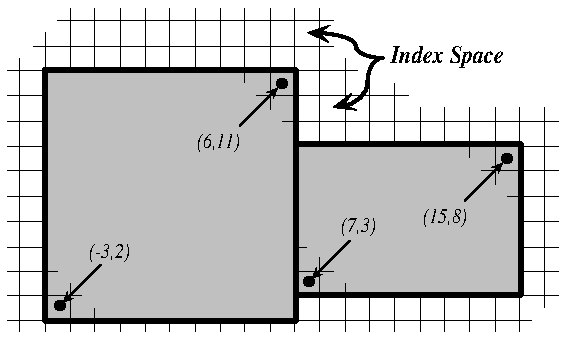
\includegraphics[width=.5\textwidth]{figStructGridBoxes}
\caption{%
A box is a collection of abstract cell-centered indices, described by its
minimum and maximum indices.  Here, two boxes are illustrated.}
\label{fig-struct-boxes}
\end{figure}
The integers may have any value, negative or positive.  The global indexes
allow \hypre{} to discern how data is related spatially, and how it is
distributed across the parallel machine.  The basic component of the grid is a
{\em box}: a collection of abstract cell-centered indices in index space,
described by its ``lower'' and ``upper'' corner indices.  The scalar grid data
is always associated with cell centers, unlike the more general \code{SStruct}
interface which allows data to be associated with box indices in several
different ways.

Each process describes that portion of the grid that it ``owns'', one box at a
time.  For example, the global grid in Figure~\ref{fig-struct-example} can be
described in terms of three boxes, two owned by process 0, and one owned by
process 1.  Figure~\ref{fig-struct-grid} shows the code for setting up the grid
on process 0 (the code for process 1 is similar).
\begin{figure}
\centering
\begin{tabular}{@{}c@{}}
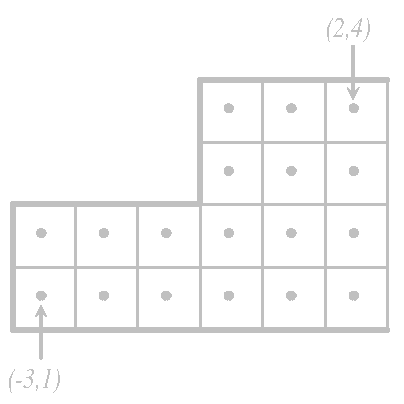
\includegraphics[width=.22\textwidth]{figStructGrid1}\vspace{-.5em} \\ 1
\end{tabular}
\hfill
\begin{tabular}{@{}c@{}}
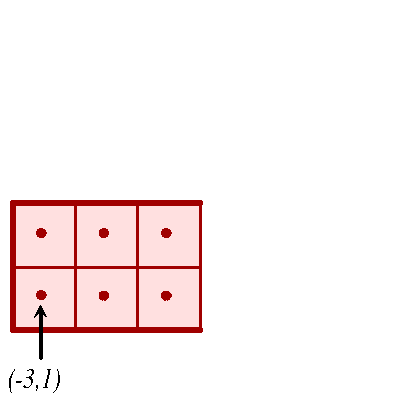
\includegraphics[width=.22\textwidth]{figStructGrid2}\vspace{-.5em} \\ 2
\end{tabular}
\hfill
\begin{tabular}{@{}c@{}}
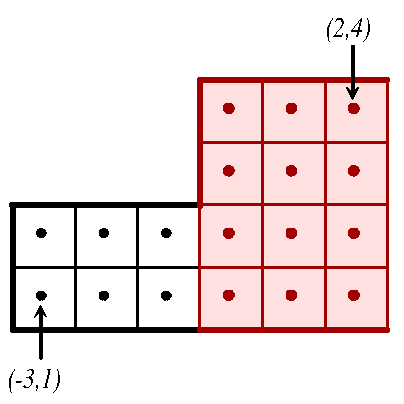
\includegraphics[width=.22\textwidth]{figStructGrid3}\vspace{-.5em} \\ 3
\end{tabular}
\hfill
\begin{tabular}{@{}c@{}}

\includegraphics[width=.22\textwidth]{figStructGrid4}\vspace{-.5em} \\ 4
\end{tabular}
\vspace{2em} \\
\begin{minipage}{0.7\textwidth}
\begin{verbatim}
   
    HYPRE_StructGrid grid;
    int ndim        = 2;
    int ilower[][2] = {{-3,1}, {0,1}};
    int iupper[][2] = {{-1,2}, {2,4}};
   
    /* Create the grid object */
1:  HYPRE_StructGridCreate(MPI_COMM_WORLD, ndim, &grid);
    
    /* Set grid extents for the first box */
2:  HYPRE_StructGridSetExtents(grid, ilower[0], iupper[0]);
    
    /* Set grid extents for the second box */
3:  HYPRE_StructGridSetExtents(grid, ilower[1], iupper[1]);
    
    /* Assemble the grid */
4:  HYPRE_StructGridAssemble(grid);
    
\end{verbatim}
\end{minipage}
\caption{%
Code on process 0 for setting up the grid in Figure~\ref{fig-struct-example}.}
\label{fig-struct-grid}
\end{figure}
The ``icons'' at the top of the figure illustrate the result of the numbered
lines of code.  The \code{Create()} routine creates an empty 2D grid object
that lives on the \code{MPI_COMM_WORLD} communicator.  The \code{SetExtents()}
routine adds a new box to the grid.  The \code{Assemble()} routine is a
collective call (i.e., must be called on all processes from a common
synchronization point), and finalizes the grid assembly, making the grid
``ready to use''.

%-----------------------------------------------------------------------------

\section{Setting Up the Struct Stencil}
\label{sec-Struct-Stencil}

The geometry of the discretization stencil is described by an array of indexes,
each representing a relative offset from any given gridpoint on the grid.  For
example, the geometry of the 5-pt stencil for the example problem being
considered can be represented by the list of index offsets shown in
Figure~\ref{fig-struct-stencil-a}.
\begin{figure}
\centering
\mbox{}\hfill
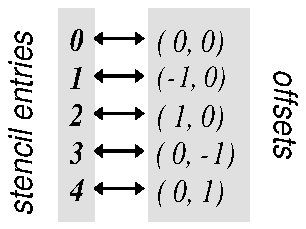
\includegraphics[width=.3\textwidth]{figStructStenc0}
\hfill
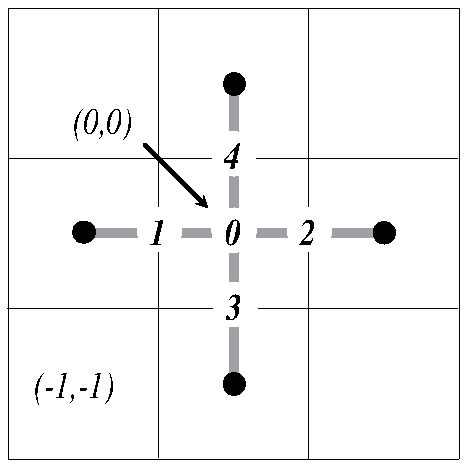
\includegraphics[width=.25\textwidth]{figStructStenc7}
\hfill\mbox{}
\caption{%
Representation of the 5-point discretization stencil for the example problem.}
\label{fig-struct-stencil-a}
\end{figure}
Here, the $(0,0)$ entry represents the ``center'' coefficient, and is the 0th
stencil entry.  The $(0,-1)$ entry represents the ``south'' coefficient, and is
the 3rd stencil entry.  And so on.

On process 0 or 1, the code in Figure~\ref{fig-struct-stencil-b} will set up
the stencil in Figure~\ref{fig-struct-stencil-a}.  The stencil must be the same
on all processes.
\begin{figure}
\centering
\mbox{}\hfill
\begin{tabular}{@{}c@{}}
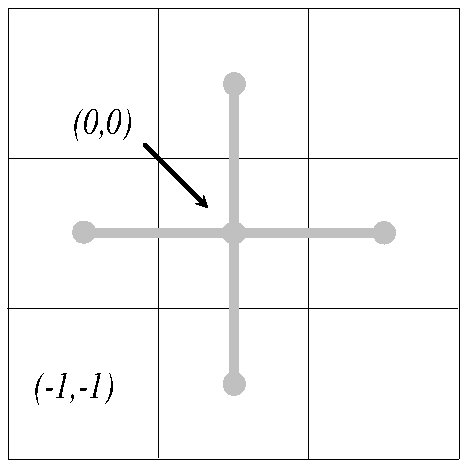
\includegraphics[width=.22\textwidth]{figStructStenc1} \\ 1
\end{tabular}
\hfill
\begin{tabular}{@{}c@{}}
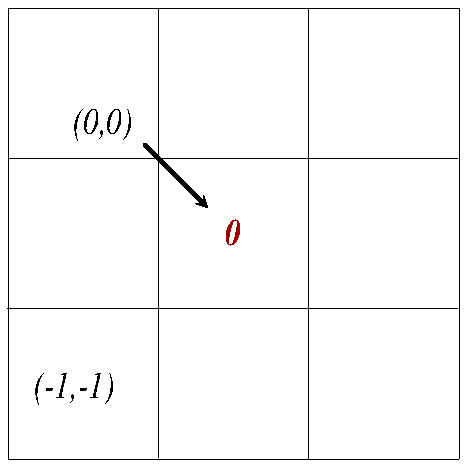
\includegraphics[width=.22\textwidth]{figStructStenc2} \\ 2
\end{tabular}
\hfill
\begin{tabular}{@{}c@{}}
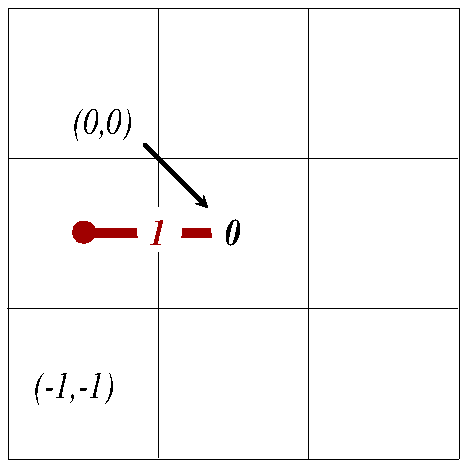
\includegraphics[width=.22\textwidth]{figStructStenc3} \\ 3
\end{tabular}
\hfill\mbox{}
\vspace{1em} \\
\mbox{}\hfill
\begin{tabular}{@{}c@{}}
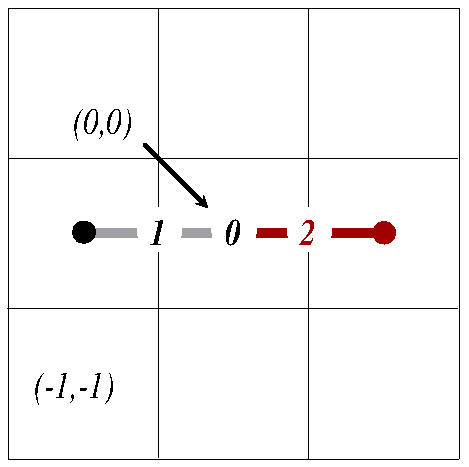
\includegraphics[width=.22\textwidth]{figStructStenc4} \\ 4
\end{tabular}
\hfill
\begin{tabular}{@{}c@{}}
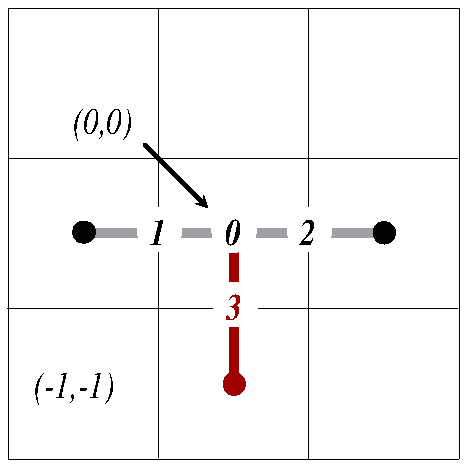
\includegraphics[width=.22\textwidth]{figStructStenc5} \\ 5
\end{tabular}
\hfill
\begin{tabular}{@{}c@{}}
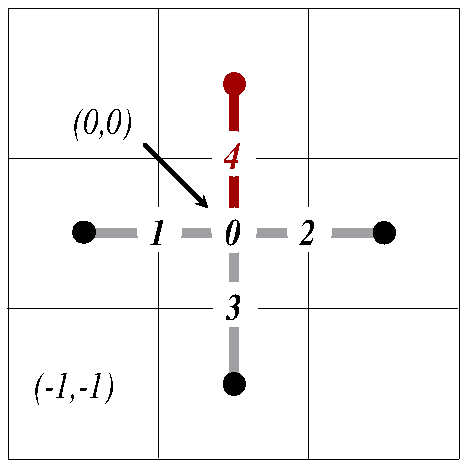
\includegraphics[width=.22\textwidth]{figStructStenc6} \\ 6
\end{tabular}
\hfill\mbox{}
\vspace{2em} \\
\begin{minipage}{0.85\textwidth}
\begin{verbatim}
      
      HYPRE_StructStencil stencil;
      int ndim         = 2;
      int size         = 5;
      int entry;
      int offsets[][2] = {{0,0}, {-1,0}, {1,0}, {0,-1}, {0,1}};
      
      /* Create the stencil object */
  1:  HYPRE_StructStencilCreate(ndim, size, &stencil);
      
      /* Set stencil entries */
      for (entry = 0; entry < size; entry++)
      {
2-6:     HYPRE_StructStencilSetElement(stencil, entry, offsets[entry]);
      }
      
      /* Thats it!  There is no assemble routine */
      
\end{verbatim}
\end{minipage}
\caption{%
Code for setting up the stencil in Figure~\ref{fig-struct-stencil-a}.}
\label{fig-struct-stencil-b}
\end{figure}
The \code{Create()} routine creates an empty 2D, 5-pt stencil object.  The
\code{SetElement()} routine defines the geometry of the stencil and assigns the
stencil numbers for each of the stencil entries.  None of the calls are
collective calls.

%-----------------------------------------------------------------------------

\section{Setting Up the Struct Matrix}
\label{sec-Struct-Matrix}

The matrix is set up in terms of the grid and stencil objects described in
Sections \ref{sec-Struct-Grid} and \ref{sec-Struct-Stencil}.  The coefficients
associated with each stencil entry will typically vary from gridpoint to
gridpoint, but in the example problem being considered, they are as follows
over the entire grid (except at boundaries; see below):
\begin{equation}\label{eqn-stencil-laplacian}
\left [
\begin{array}{ccc}
    & -1 &    \\
 -1 &  4 & -1 \\
    & -1 &    
\end{array}
\right ] .
\end{equation}

On process 0, the code in Figure~\ref{fig-struct-matrix} will set up matrix
values associated with the center (entry 0) and south (entry 3) stencil entries
as given by \ref{eqn-stencil-laplacian} and Figure~\ref{fig-struct-matrix}
(boundaries are ignored here temporarily).
\begin{figure}
\centering
\begin{minipage}{0.75\textwidth}
\begin{verbatim}

HYPRE_StructMatrix  A;
double              values[36];
int                 stencil_indices[2] = {0,3};
int                 i;

HYPRE_StructMatrixCreate(MPI_COMM_WORLD, grid, stencil, &A);
HYPRE_StructMatrixInitialize(A);

for (i = 0; i < 36; i += 2)
{
   values[i]   =  4.0;
   values[i+1] = -1.0;
}

HYPRE_StructMatrixSetBoxValues(A, ilower[0], iupper[0], 2,
                               stencil_indices, values);
HYPRE_StructMatrixSetBoxValues(A, ilower[1], iupper[1], 2,
                               stencil_indices, values);

/* set boundary conditions */
...

HYPRE_StructMatrixAssemble(A);

\end{verbatim}
\end{minipage}
\caption{%
Code for setting up matrix values associated with stencil entries 0 and 3 as
given by \ref{eqn-stencil-laplacian} and Figure~\ref{fig-struct-stencil-a}.}
\label{fig-struct-matrix}
\end{figure}
The \code{Create()} routine creates an empty matrix object.  The
\code{Initialize()} routine indicates that the matrix coefficients (or values)
are ready to be set.  This routine may or may not involve the allocation of
memory for the coefficient data, depending on the implementation.  The optional
\code{Set} routines mentioned later in this chapter and in the Reference
Manual, should be called before this step.  The \code{SetBoxValues()} routine
sets the matrix coefficients for some set of stencil entries over the
gridpoints in some box.  Note that the box need not correspond to any of the
boxes used to create the grid, but values should be set for all gridpoints that
this process ``owns''.  The \code{Assemble()} routine is a collective call, and
finalizes the matrix assembly, making the matrix ``ready to use''.

Matrix coefficients that reach outside of the boundary should be set to zero.
For efficiency reasons, \hypre{} does not do this automatically.  The most
natural time to insure this is when the boundary conditions are being set, and
this is most naturally done after the coefficients on the grid's interior have
been set.  For example, during the implementation of the Dirichlet boundary
condition on the lower boundary of the grid in Figure~\ref{fig-struct-example},
the ``south'' coefficient must be set to zero.  To do this on process 0, the
code in Figure~\ref{fig-struct-matrix-boundary} could be used:
\begin{figure}
\centering
\begin{minipage}{0.8\textwidth}
\begin{verbatim}

int  ilower[2] = {-3, 1};
int  iupper[2] = { 2, 1};

/* create matrix and set interior coefficients */
...

/* implement boundary conditions */
...

for (i = 0; i < 12; i++)
{
   values[i] =  0.0;
}

i = 3;
HYPRE_StructMatrixSetBoxValues(A, ilower, iupper, 1, &i, values);

/* complete implementation of boundary conditions */
...

\end{verbatim}
\end{minipage}
\caption{%
Code for adjusting boundary conditions along the lower grid boundary in
Figure~\ref{fig-struct-example}.}
\label{fig-struct-matrix-boundary}
\end{figure}

%-----------------------------------------------------------------------------

\section{Setting Up the Struct Right-Hand-Side Vector}
\label{sec-Struct-RHS}

The right-hand-side vector is set up similarly to the matrix set up described
in Section \ref{sec-Struct-Matrix} above.  The main difference is that there is
no stencil (note that a stencil currently does appear in the interface, but
this will eventually be removed).

On process 0, the code in Figure~\ref{fig-struct-rhs} will set up the
right-hand-side vector values.
\begin{figure}
\centering
\begin{minipage}{0.8\textwidth}
\begin{verbatim}

HYPRE_StructVector  b;
double              values[18];
int                 i;

HYPRE_StructVectorCreate(MPI_COMM_WORLD, grid, &b);
HYPRE_StructVectorInitialize(b);

for (i = 0; i < 18; i++)
{
   values[i]   =  0.0;
}

HYPRE_StructVectorSetBoxValues(b, ilower[0], iupper[0], values);
HYPRE_StructVectorSetBoxValues(b, ilower[1], iupper[1], values);

HYPRE_StructVectorAssemble(b);

\end{verbatim}
\end{minipage}
\caption{%
Code for setting up right-hand-side vector values.}
\label{fig-struct-rhs}
\end{figure}
The \code{Create()} routine creates an empty vector object.  The
\code{Initialize()} routine indicates that the vector coefficients (or values)
are ready to be set.  This routine follows the same rules as its corresponding
\code{Matrix} routine.  The \code{SetBoxValues()} routine sets the vector
coefficients over the gridpoints in some box, and again, follows the same rules
as its corresponding \code{Matrix} routine.  The \code{Assemble()} routine is a
collective call, and finalizes the vector assembly, making the vector ``ready
to use''.

%-----------------------------------------------------------------------------

\section{Symmetric Matrices}
\label{sec-Symmetric-Matrices}

Some solvers and matrix storage schemes provide capabilities for significantly
reducing memory usage when the coefficient matrix is symmetric.  In this
situation, each off-diagonal coefficient appears twice in the matrix, but only
one copy needs to be stored.  The \code{Struct} interface provides support for
matrix and solver implementations that use symmetric storage via the
\code{SetSymmetric()} routine.

To describe this in more detail, consider again the 5-pt finite-volume
discretization of (\ref{eqn-laplacian}) on the grid pictured in
Figure~\ref{fig-struct-example}.  Because the discretization is symmetric, only
half of the off-diagonal coefficients need to be stored.  To turn symmetric
storage on, the following line of code needs to be inserted somewhere between
the \code{Create()} and \code{Initialize()} calls.
\begin{display}
\begin{verbatim}

HYPRE_StructMatrixSetSymmetric(A, 1);

\end{verbatim}
\end{display}
The coefficients for the entire stencil can be passed in as before.  Note that
symmetric storage may or may not actually be used, depending on the underlying
storage scheme.  Currently in \hypre{}, the \code{Struct} interface always uses
symmetric storage.

To most efficiently utilize the \code{Struct} interface for symmetric matrices,
notice that only half of the off-diagonal coefficients need to be set.  To do
this for the example being considered, we simply need to redefine the 5-pt
stencil of Section \ref{sec-Struct-Stencil} to an ``appropriate'' 3-pt stencil,
then set matrix coefficients (as in Section \ref{sec-Struct-Matrix}) for these
three stencil elements {\em only}.  For example, we could use the following
stencil
\begin{equation}\label{eqn-symmetric-stencil}
\left [
\begin{array}{ccc}
~~~~~~ & ( 0, 1) &         \\
~~~~~~ & ( 0, 0) & ( 1, 0) \\
~~~~~~ &         &        
\end{array}
\right ] .
\end{equation}
This 3-pt stencil provides enough information to recover the full 5-pt stencil
geometry and associated matrix coefficients.
